\section{Results (Exploratory)}\label{sec:results}
\emph{All numbers below are descriptive, from 321 non-pristine development pairs, post-fix. They are not evidence of performance in the field. Every table names its source file.}

\textbf{Overall metrics.} Table~\ref{tab:metrics} gives the system metrics. V7-B detects 0.708 of the divergent-labelled pairs (75 \DIV, 13 \NDO, 18 \INS), B1 0.774 (82/24/0), and B3 0.811. B1 detected every pair that V7-B detected (no pair is \DIV{} for V7-B and not for B1; 55 pairs are \DIV{} for B1 and not for V7-B, mostly renamed-entry pairs that V7-B refuses). V7-B's false-alarm rate on no-difference-labelled pairs is 0.000, against about 0.30 for B1, B1+rep and B3; all 46 B1 false alarms are renamed-entry pairs, a harness artefact rather than a behavioural false alarm. Without the renamed-entry pairs (sensitivity run, \path{results/postfix/statistics/sensitivity_excluding_SP2_renamed/system_metrics.csv}) B1 false alarm is 0.000, detection is 0.767 for B1 against 0.728 for V7-B, and V7-B abstention is 0.203.
\begin{table*}[t]
\centering\scriptsize
\caption{Descriptive metrics, 95\% project-cluster bootstrap CI (B=10000, seed 42), post-fix run. Exploratory; non-pristine development data. Source: \path{results/postfix/statistics/system_metrics.csv}, \path{results/postfix/statistics/cost.csv}.}
\label{tab:metrics}
\begin{tabular}{lrrrrr}
\hline
System & Detection (DIV) & False assur. (DIV) & Abstention & False alarm & CPU s median (sum) \\
\hline
V7-B & 0.708 [0.545, 0.816] & 0.123 [0.054, 0.236] & 0.360 [0.306, 0.435] & 0.000 [0.000, 0.000] & 1.30 (456) \\
B1 & 0.774 [0.609, 0.881] & 0.226 [0.119, 0.392] & 0.000 [0.000, 0.000] & 0.303 [0.149, 0.352] & 0.40 (151) \\
B1+rep & 0.774 [0.610, 0.880] & 0.226 [0.120, 0.390] & 0.000 [0.000, 0.000] & 0.303 [0.148, 0.352] & 1.26 (543) \\
B3 & 0.811 [0.662, 0.904] & 0.189 [0.097, 0.337] & 0.000 [0.000, 0.000] & 0.309 [0.147, 0.361] & 3.77 (1424) \\
B4 & 0.009 [0.000, 0.019] & 0.991 [0.981, 1.000] & 0.000 [0.000, 0.000] & 0.007 [0.000, 0.010] & 0.00 (0) \\
\hline
\end{tabular}
\end{table*}

\begin{figure}[t]\centering
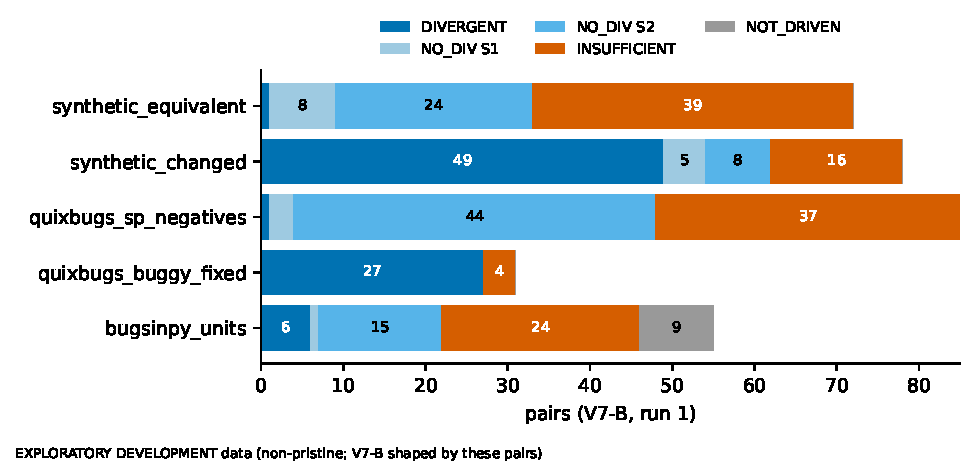
\includegraphics[width=\columnwidth]{../../results/postfix/figures/fig_verdict_sufficiency_by_dataset.pdf}
\caption{V7-B verdict and sufficiency per dataset (post-fix; source \path{results/postfix/figures/}, generated by \texttt{scripts/generate\_figures.py}). The earlier pre-fix versions are in \path{results/figures/} and are superseded.}\label{fig:verdictds}
\end{figure}
Table~\ref{tab:byarm} gives the verdict distribution per arm.
\begin{table}[t]
\centering\scriptsize
\caption{V7-B verdict and level per arm, all pairs including suspect and unlabelled (post-fix). Source: \path{paper/IEEE_ACCESS_INITIAL_MANUSCRIPT/tables/derived_crosstab.csv}.}
\label{tab:byarm}
\begin{tabular}{lrrrrr}
\hline
Arm & DIVERGENT & S2 & S1 & INSUFF. & Not driven \\
\hline
quixbugs\_buggy\_fixed & 27 & 0 & 0 & 4 & 0 \\
quixbugs\_sp\_negatives & 1 & 44 & 3 & 37 & 0 \\
synthetic\_changed & 49 & 8 & 5 & 16 & 0 \\
synthetic\_equivalent & 1 & 24 & 8 & 39 & 0 \\
bugsinpy\_units & 6 & 15 & 1 & 24 & 9 \\
\hline
\end{tabular}
\end{table}


\textbf{Paired comparison.} Table~\ref{tab:paired} compares against B1. V7-B has a lower false-assurance rate (improvement 0.104) but this is mostly outcomes relocating to \INS: V7-B abstains on 18 divergent-labelled pairs, and the lower detection (difference $-0.066$, 7 pairs in which only B1 succeeds, none the other way) is not significant after Holm correction. No row satisfies the +10pp rule. Matched-coverage false assurance (gate K4) was not computed, so these rows do not support any superiority claim. B3 detects four more pairs than B1 by mutation, a difference that is not significant.
\begin{table*}[t]
\centering\scriptsize
\caption{Paired comparisons against B1 (improvement is positive when better; b = test-only, c = reference-only successes). Unadjusted exploratory; no row meets the +10pp rule. Source: \path{results/postfix/statistics/paired_comparisons.csv}.}
\label{tab:paired}
\begin{tabular}{lrrrrrrrr}
\hline
Test & Outcome & Improv. & 95\% CI & b & c & p sign-flip & p Holm & +10pp \\
\hline
B1+rep & false assurance & -0.000 & [-0.000, -0.000] & 0 & 0 & 1.000 & 1.000 & False \\
B1+rep & detection & 0.000 & [0.000, 0.000] & 0 & 0 & 1.000 & 1.000 & False \\
B3 & false assurance & 0.038 & [0.007, 0.090] & 0 & 4 & 0.125 & 0.500 & False \\
B3 & detection & 0.038 & [0.007, 0.090] & 4 & 0 & 0.125 & 0.500 & False \\
V7-B & false assurance & 0.104 & [0.043, 0.205] & 0 & 11 & 0.001 & 0.006 & False \\
V7-B & detection & -0.066 & [-0.115, -0.026] & 0 & 7 & 0.031 & 0.156 & False \\
\hline
\end{tabular}
\end{table*}


\textbf{Negative finding 1: replay adds nothing measurable (B1+rep $\approx$ B1).} B1+rep equals B1 on all primary outcomes (zero discordant pairs in Table~\ref{tab:paired}). Over all 321 pairs the two differ on exactly 2 (B1 \DIV, B1+rep \texttt{NO\_DIFF}), both nondeterminism cases that V7-B reports as \INS{} (nondeterministic): a synthetic pair with a suspect label and a BugsInPy unit. The machinery of $r_{replay}=5$ and $k_{alt}=3$ shows no measurable value over repetition on these data, and the independent reviewer saw no witness demoted to environment-sensitive. V7-B costs roughly three times B1's CPU (Table~\ref{tab:metrics}).

\textbf{Negative finding 2: sufficiency does not visibly separate labels.} On synthetic pairs where B1 saw no difference, if sufficiency carried signal, S2 should be markedly purer in no-difference labels than \INS. Table~\ref{tab:suffsep} shows the shares are close (S2 holds 8 changed and 24 equivalent; \INS{} holds 11 and 23) and the direction for S1 is wrong. Labels are noisy and counts small, so this is not proof either way, but it is the only data and it is not supportive. Further, 16 of the 46 driven BugsInPy units, which are real fixes, received \NDO{} (15 at S2) on a synthetic battery, and 13 of 78 changed-labelled synthetic pairs received \NDO{}; S2 does not stop this failure mode.
\begin{table}[t]
\centering\scriptsize
\caption{V7-B outcome on synthetic pairs where B1 saw no difference, by generator label (suspect labels included, as in the red-team analysis). If sufficiency separated labels, S2 would be purer in EQUIVALENT than INSUFFICIENT; it is not clearly so. Source: \path{paper/IEEE_ACCESS_INITIAL_MANUSCRIPT/tables/derived_crosstab.csv}.}
\label{tab:suffsep}
\begin{tabular}{lrrr}
\hline
Generator label & V7-B S2 & V7-B S1 & V7-B INSUFFICIENT \\
\hline
CHANGED & 8 & 5 & 11 \\
EQUIVALENT & 24 & 8 & 23 \\
\hline
\end{tabular}
\end{table}


\textbf{Risk--coverage.} Table~\ref{tab:riskcov} and Fig.~\ref{fig:riskcov} show V7-B deciding fewer pairs (coverage 0.640 at all levels) with lower risk (0.079) than baselines that decide every pair (risk 0.271 for B1). Restricting to S2 lowers coverage and risk slightly. Risk is against generator labels with known defects, baselines have no sufficiency level, and this is a descriptive curve, not matched-coverage superiority.
\begin{table}[t]
\centering\scriptsize
\caption{Risk--coverage against generator labels. Baselines carry no sufficiency level, so their S-level rows are not comparable; V7-B at S3 is empty because S3 is never emitted. Source: \path{results/postfix/statistics/risk_coverage.csv}.}
\label{tab:riskcov}
\begin{tabular}{lrrrrr}
\hline
System & Min. level & Coverage & Risk & Decided & Eligible \\
\hline
B1 & none & 1.000 & 0.271 & 258 & 258 \\
B1 & S2 & 0.496 & 0.359 & 128 & 258 \\
B1 & S3 & 0.496 & 0.359 & 128 & 258 \\
B1+rep & none & 1.000 & 0.271 & 258 & 258 \\
B1+rep & S2 & 0.496 & 0.359 & 128 & 258 \\
B1+rep & S3 & 0.496 & 0.359 & 128 & 258 \\
B3 & none & 1.000 & 0.260 & 258 & 258 \\
B3 & S2 & 0.516 & 0.353 & 133 & 258 \\
B3 & S3 & 0.516 & 0.353 & 133 & 258 \\
V7-B & none & 0.640 & 0.079 & 165 & 258 \\
V7-B & S2 & 0.578 & 0.054 & 149 & 258 \\
V7-B & S3 & 0.291 & 0.000 & 75 & 258 \\
\hline
\end{tabular}
\end{table}

\begin{figure}[t]\centering
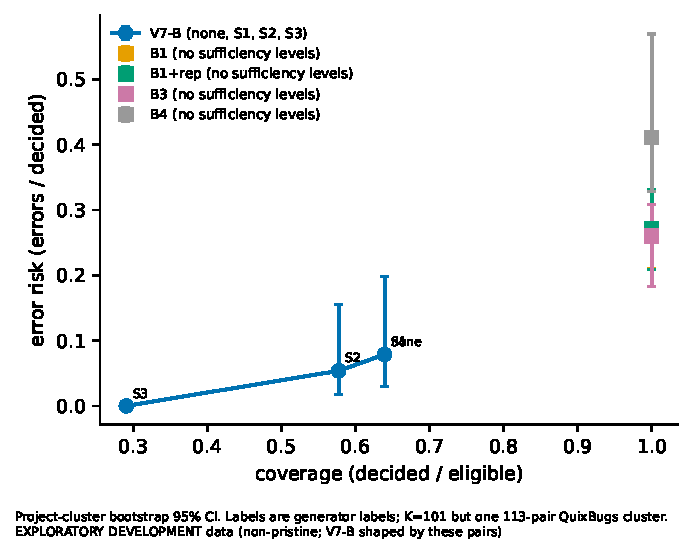
\includegraphics[width=\columnwidth]{../../results/postfix/figures/fig_risk_coverage.pdf}
\caption{Coverage versus error risk (post-fix; descriptive; generator labels; source \path{results/postfix/figures/}).}\label{fig:riskcov}
\end{figure}

\textbf{QuixBugs.} V7-B detected 27 of the 29 test-witnessed pairs (4 \INS: two loop forever in the buggy version, two are generator functions); B1, B1+rep and B3 detected 29 of 29; the edit-size heuristic B4 detected 1. There is no cluster interval because QuixBugs is one cluster (Fig.~\ref{fig:quix}).
\begin{figure}[t]\centering
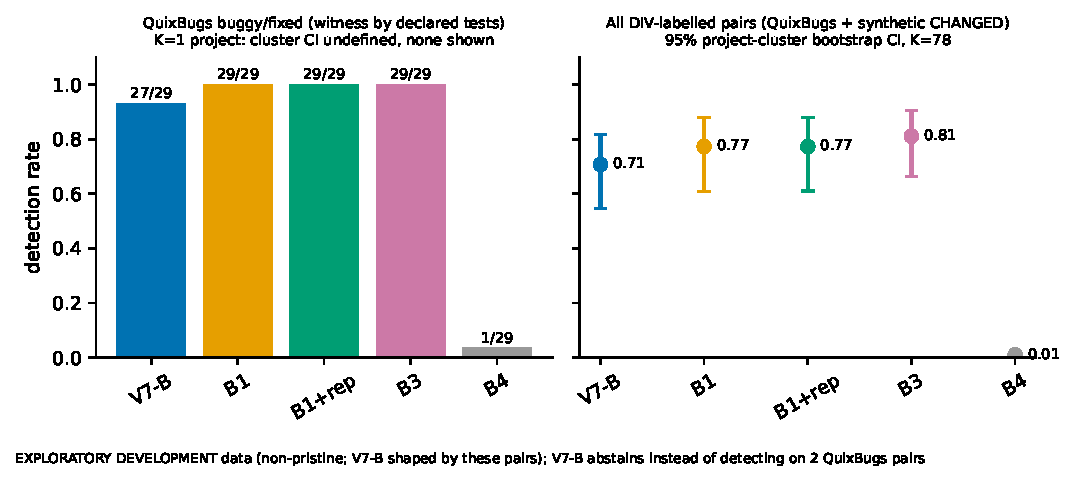
\includegraphics[width=\columnwidth]{../../results/postfix/figures/fig_detection_quixbugs_vs_baselines.pdf}
\caption{Detection on QuixBugs (one cluster) and on all divergent-labelled pairs with cluster intervals (source \path{results/postfix/figures/}); no superiority claim.}\label{fig:quix}
\end{figure}

\textbf{Class counts and runtime.} Table~\ref{tab:classcounts} lists verdict counts by truth class for V7-B and B1. Fig.~\ref{fig:runtime} shows CPU per pair; V7-B CPU is child-process time only and is a lower bound; memory was not recorded.
\begin{table}[t]
\centering\scriptsize
\caption{Verdict counts by truth class for V7-B and B1 (post-fix). Source: \path{results/postfix/statistics/class_counts.csv}.}
\label{tab:classcounts}
\begin{tabular}{lrrr}
\hline
System & Truth & Verdict & n \\
\hline
B1 & DIV & DIVERGENT\_OBSERVABLE & 82 \\
B1 & DIV & NO\_DIVERGENCE\_OBSERVED & 24 \\
B1 & NO\_OBS\_DIFF & DIVERGENT\_OBSERVABLE & 46 \\
B1 & NO\_OBS\_DIFF & NO\_DIVERGENCE\_OBSERVED & 106 \\
V7-B & DIV & DIVERGENT\_OBSERVABLE & 75 \\
V7-B & DIV & INSUFFICIENT & 18 \\
V7-B & DIV & NO\_DIVERGENCE\_OBSERVED & 13 \\
V7-B & NO\_OBS\_DIFF & INSUFFICIENT & 75 \\
V7-B & NO\_OBS\_DIFF & NO\_DIVERGENCE\_OBSERVED & 77 \\
\hline
\end{tabular}
\end{table}

\begin{figure}[t]\centering
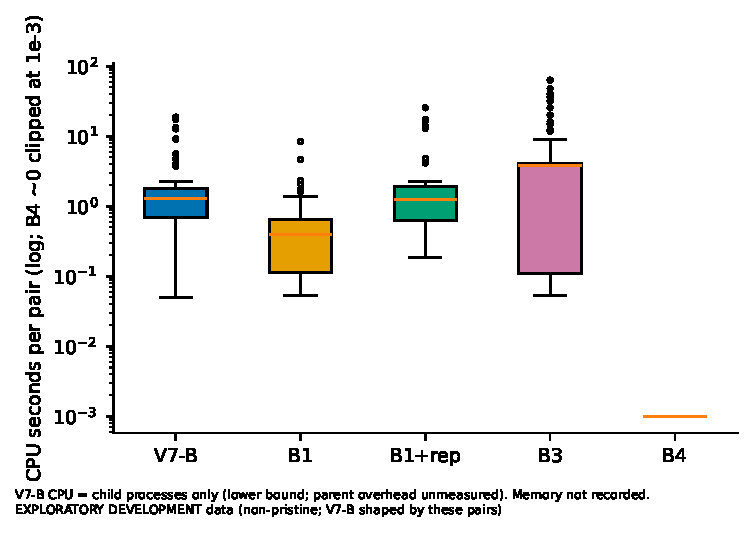
\includegraphics[width=\columnwidth]{../../results/postfix/figures/fig_runtime.pdf}
\caption{CPU seconds per pair per system, log scale (post-fix; V7-B child CPU only).}\label{fig:runtime}
\end{figure}

\textbf{Power.} Table~\ref{tab:power} shows that on the observed design (78 clusters, 106 pairs, discordance 0.066) power at +5pp is at most 0.27, and +10pp is not reachable because the observed discordance cannot carry a 10pp difference. This design cannot support a confirmatory claim.
\begin{table}[t]
\centering\scriptsize
\caption{Simulated power on the observed development design (K=78, 106 pairs, discordance 0.066); simulation assumptions A1--A4 are in the source file; not a prediction of system performance. Source: \path{results/postfix/statistics/power_actual.json}.}
\label{tab:power}
\begin{tabular}{lrrr}
\hline
ICC rho & alpha & Power +5pp & Power +10pp \\
\hline
0.0 & 0.05 & 0.267 & not reachable \\
0.0 & 0.0167 & 0.123 & not reachable \\
0.05 & 0.05 & 0.247 & not reachable \\
0.05 & 0.0167 & 0.095 & not reachable \\
0.15 & 0.05 & 0.215 & not reachable \\
0.15 & 0.0167 & 0.085 & not reachable \\
0.3 & 0.05 & 0.227 & not reachable \\
0.3 & 0.0167 & 0.068 & not reachable \\
\hline
\end{tabular}
\end{table}


\textbf{Determinism and crashes.} Whole-pair re-runs gave identical verdicts, levels, reasons and witness ids on every re-run pair (Table~\ref{tab:k1}); all 321 invocations produced a verdict with no engine crash. This shows the harness is stable on development pairs, not that verdicts are correct.
\begin{table}[t]
\centering\scriptsize
\caption{K1 spike per-arm counts and whole-pair re-run determinism (post-fix; the synthetic arm was not re-run after the fix). K1 itself is NOT MET. Source: \path{results/postfix/processed/k1_spike_summary.json}.}
\label{tab:k1}
\begin{tabular}{lrrrrr}
\hline
Arm & Pairs & Runnable & Projects & Re-run & Identical \\
\hline
quixbugs & 31 & 30 & 1 & 31 & 31 \\
quixbugs\_neg & 85 & 54 & 1 & 25 & 25 \\
synthetic & 150 & 132 & 101 & 0 & 0 \\
bugsinpy\_units & 55 & 44 & 12 & 46 & 46 \\
\hline
\end{tabular}
\end{table}

